
\documentclass[journal]{vgtc}                % final (journal style)
%\documentclass[review,journal]{vgtc}         % review (journal style)
%\documentclass[widereview]{vgtc}             % wide-spaced review
%\documentclass[preprint,journal]{vgtc}       % preprint (journal style)

%% Uncomment one of the lines above depending on where your paper is
%% in the conference process. ``review'' and ``widereview'' are for review
%% submission, ``preprint'' is for pre-publication, and the final version
%% doesn't use a specific qualifier.

%% Please use one of the ``review'' options in combination with the
%% assigned online id (see below) ONLY if your paper uses a double blind
%% review process. Some conferences, like IEEE Vis and InfoVis, have NOT
%% in the past.

%% Please note that the use of figures other than the optional teaser is not permitted on the first page
%% of the journal version.  Figures should begin on the second page and be
%% in CMYK or Grey scale format, otherwise, colour shifting may occur
%% during the printing process.  Papers submitted with figures other than the optional teaser on the
%% first page will be refused. Also, the teaser figure should only have the
%% width of the abstract as the template enforces it.

%% These few lines make a distinction between latex and pdflatex calls and they
%% bring in essential packages for graphics and font handling.
%% Note that due to the \DeclareGraphicsExtensions{} call it is no longer necessary
%% to provide the the path and extension of a graphics file:
%% 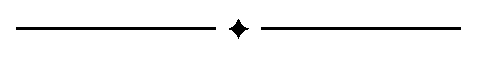
\includegraphics{diamondrule} is completely sufficient.
%%
\ifpdf%                                % if we use pdflatex
  \pdfoutput=1\relax                   % create PDFs from pdfLaTeX
  \pdfcompresslevel=9                  % PDF Compression
  \pdfoptionpdfminorversion=7          % create PDF 1.7
  \ExecuteOptions{pdftex}
  \usepackage{graphicx}                % allow us to embed graphics files
  \DeclareGraphicsExtensions{.pdf,.png,.jpg,.jpeg} % for pdflatex we expect .pdf, .png, or .jpg files
\else%                                 % else we use pure latex
  \ExecuteOptions{dvips}
  \usepackage{graphicx}                % allow us to embed graphics files
  \DeclareGraphicsExtensions{.eps}     % for pure latex we expect eps files
\fi%

%% it is recomended to use ``\autoref{sec:bla}'' instead of ``Fig.~\ref{sec:bla}''
\graphicspath{{figures/}{pictures/}{images/}{./}} % where to search for the images

\usepackage{microtype}                 % use micro-typography (slightly more compact, better to read)
\PassOptionsToPackage{warn}{textcomp}  % to address font issues with \textrightarrow
\usepackage{textcomp}                  % use better special symbols
\usepackage{mathptmx}                  % use matching math font
\usepackage{times}                     % we use Times as the main font
\renewcommand*\ttdefault{txtt}         % a nicer typewriter font
\usepackage{cite}                      % needed to automatically sort the references
\usepackage{tabu}                      % only used for the table example
\usepackage{booktabs}                  % only used for the table example
%% We encourage the use of mathptmx for consistent usage of times font
%% throughout the proceedings. However, if you encounter conflicts
%% with other math-related packages, you may want to disable it.
\usepackage{wrapfig}
\usepackage{subfig}
\usepackage{caption}

\usepackage{hyperref}
\usepackage[usenames, dvipsnames]{color}
%% In preprint mode you may define your own headline.
%\preprinttext{To appear in IEEE Transactions on Visualization and Computer Graphics.}

%% If you are submitting a paper to a conference for review with a double
%% blind reviewing process, please replace the value ``0'' below with your
%% OnlineID. Otherwise, you may safely leave it at ``0''.
\onlineid{0}

%% declare the category of your paper, only shown in review mode
\vgtccategory{Research}
%% please declare the paper type of your paper to help reviewers, only shown in review mode
%% choices:
%% * algorithm/technique
%% * application/design study
%% * evaluation
%% * system
%% * theory/model
\vgtcpapertype{algorithm/technique}

\newcommand\addcomment[1]{\textcolor{red}{#1}}

\newcommand{\specialcell}[2][l]{%
\begin{tabular}[#1]{@{}l@{}}#2\end{tabular}}

%% Paper title.
%\title{Data-Driven Animation Effect Enhancement to Activate Static Visual Charts}
\title{City Folding: Visual Exploration of Urban Dynamics based on Diverse Deomgraphics}

%U-topia: 

%City Folding: Visual Exploration of Urban Dynamics based on Diverse Deomgraphics Data Collected via Social Media

% City Folding: A Map Distortion Method Driven by Social Deomgraphics Data

% Visual Exploration of Urban Demographic Visual Exploration of Urban Data


%% This is how authors are specified in the journal style

%% indicate IEEE Member or Student Member in form indicated below
%\author{Qi Wang, Min Lu, Yang Yue, ...}
%\authorfooter{
%% insert punctuation at end of each item
%\item
%Qi Wang, Min Lu and Hui Huang are with Shenzhen University. E-mail: \{minlu, huihuang\}@szu.edu.cn
%\item
% Noa Fish is with Tel Aviv University, E-mail: {noafish}@post.tau.ac.il
%\item
%Dainel Cohen-Or is with Tel Aviv University and Shenzhen University, E-mail: {dcor}@tau.ac.il
%\item 
%To whom correspondence should be addressed,
%email: {huihuang}@szu.edu.cn
%}

%other entries to be set up for journal
%\shortauthortitle{Lu \MakeLowercase{\textit{et al.}}: Enhancing Static Visual Charts}
%\shortauthortitle{Firstauthor \MakeLowercase{\textit{et al.}}: Paper Title}

%% Abstract section.
\abstract{A city is shaped not only by its natural geographic landscape but also by social accessiblity to various citizens. In this work, via a social wide census investigation via the social media platform, citizens with various demographics are reached. We propose a visual analytics system to provide an intuitive perception of the accessiblity and activity, i.e., the kind of city folding phenomenon, in the context of various levels of social attributes (e.g., income, education, etc). Accompanied with temporal and spatial multiple views, the method is capable to reveal the detail of levels.%
} % end of abstract

%% Keywords that describe your work. Will show as 'Index Terms' in journal
%% please capitalize first letter and insert punctuation after last keyword
\keywords{Demographics, Spatial-temporal Visualization, Map Distortion}

%% ACM Computing Classification System (CCS). 
%% See <http://www.acm.org/class/1998/> for details.
%% The ``\CCScat'' command takes four arguments.

\CCScatlist{ % not used in journal version
 \CCScat{K.6.1}{Management of Computing and Information Systems}%
{Project and People Management}{Life Cycle};
 \CCScat{K.7.m}{The Computing Profession}{Miscellaneous}{Ethics}
}

%% Uncomment below to include a teaser figure.
% \teaser{
%   \centering
%   \includegraphics[width=\linewidth]{CypressView}
%   \caption{In the Clouds: Vancouver from Cypress Mountain. Note that the teaser may not be wider than the abstract block.}
% 	\label{fig:teaser}
% }

%% Uncomment below to disable the manuscript note
%\renewcommand{\manuscriptnotetxt}{}

%% Copyright space is enabled by default as required by guidelines.
%% It is disabled by the 'review' option or via the following command:
% \nocopyrightspace

\vgtcinsertpkg

%%%%%%%%%%%%%%%%%%%%%%%%%%%%%%%%%%%%%%%%%%%%%%%%%%%%%%%%%%%%%%%%
%%%%%%%%%%%%%%%%%%%%%% START OF THE PAPER %%%%%%%%%%%%%%%%%%%%%%
%%%%%%%%%%%%%%%%%%%%%%%%%%%%%%%%%%%%%%%%%%%%%%%%%%%%%%%%%%%%%%%%%

\begin{document}

%% The ``\maketitle'' command must be the first command after the
%% ``\begin{document}'' command. It prepares and prints the title block.

%% the only exception to this rule is the \firstsection command
\firstsection{Introduction}

\maketitle

%% \section{Introduction} %for journal use above \firstsection{..} instead
%Without interference with other visual encoding, animation effect is proved as a light-weight extra and preattensive cue. 

City is shaped by accessibility. Activity of people is constrained by social attributes. City planning is to relax the space which would activate the city... (Look for some statement in paper about the importance of community diversity)

In many work, anonymous movement data reveal the overall travel behaviour without social characteristics... Urban infrastructure centered, roads, regions are studied. Peopole centered, most related work is social media based, By considering people as the mobile sensor, about certain topics/keywords it is also an indirect way. 

Because social characteristics is private that not easy to get. (Emphasize how special our research is). We conduct an online demographical colleciton campaign based on famouse social medial platform. With the wide-use of mobile device. Collecting data via a widely used social medial platform, users (what the right word here?) with various profiles are reached and assembled as rich (and fair?) demographic data. (what we are going to do)

In this work, we propose a visual analytics system People Centered. Interactive Classification Method, Movement Clustering Algorithm, A visual method about data driven semnatic visual profile drawing, 2.5 Spatial Exploration. ...



\section{Related Work}

This work concerns to the research topic of spatial data visual analytics. Spatio-temporal data has three components, i.e., spatial, temporal and thematic~\cite{andrienko2013visual}. Lots of related work focus on the spatio-temporal analysis in movement data, in the absence of thematic information. The presense of geo-tagged social media data flourishes the exploration of thematic information along with movement. By analyzing the texts, those work explain what drive the moving activities or what is resulted from. This work continues the thematic research in movement data, but focus more on individual charecteristics. Landed by a census experiment, this work is able to analyze the profile information directly, to get rid of indirect data inferred from social media data as other related work do.

\textbf{Movement Data Analysis} 
 
 With the development of location-acquistion techniques, massive spatial trajectories are collected, to keep track of the trajectories of various moving objects. Many techniques have been proposed to process, mining trajectory~\cite{Zheng2015_trajectory}. In the field of visualization and visual analytic, spatial visualizations are specifically designed for the time, locations, spatial-temporal information and other properties in the traffic data~\cite{chen2015survey}. A large number of visual analytics tools and applications cover situation-aware exploration, pattern discovery and traffic situation monitoring. Wang et al~\cite{wang2013visual} extract the traffic jam propagation graph extraction to reveal underlying data patterns. Guo et al.~\cite{guo2011tripvista} and Zeng et al.~\cite{zeng2013visualizing} et al. construct geographical regions and visually aggregate the in-between movements as flows. To discover the route travel patterns, Lu et al.~\cite{lu2015trajrank} propose TrajRank to explore the route travel behaviour based on ranking. For multiple routes, Liu et al.~\cite{liu2011_routediversity} study the route diversity between locations and Lu et al.~\cite{Lu2017_multipleroute} explore the route choice behaviour among multiple routes.


\textbf{Geo-tagged Social Media Data Analysis}

As the prevence of social medial serivces, social media data with geo-tags are collected to track people's movements in daily lifes. As an analogue of remote sensing data in social science research, the geospatial big data has been proposed as social sensing ~\cite{liu2015social}. Hence, analyzing movement information along with rich text has become a hot research area in recent years. Those works infer thematic information from the semantic texts. Cao et al.~\cite{cao2012whisper} propose \textit{Whisper} for tracing the pathways of tweets on a spatial hierarchical layouts, to investigate how information flow among multiple places. Krueger et al.~\cite{krueger2014visual} used GPS and location-based service data to support the analysis of movement behaviors. Chen et al.~\cite{chen2016interactive} present a visual analytics system to support the exploraiton of sparcely sampled trajectory from social media. Some other researches tend to infer real information, such as names, gender, etc~\cite{peddinti2014internet}, to break down the demographic characteristics of social media users. Luo et al.~\cite{luo2016explore} derive race, gender and age as three demographics dimensions to analyze its impact on the urban human mobility patterns. Since real information is not enforced in social media, wrong infering is inevitable. Longley et al.~\cite{Longley2015}~\cite{Paul2016_twitter} identifies and assess the biases inherent in social media usage in social research and evaluate the deployment of social media data in research applications.  








\section{Data}

The advent of mobile sensing techniques makes it possible to develop urban geography from social media source. Complement the conventional census, social media brings the benefit of larger sampling frequency and higher disaggregate in terms of space and time, which reaches a wide range of individuals as well as collects the movement in human inactive time, such as the mid-night.

By Wechat, a widely used social media app we deployed the data collecting experiment in Shenzhen, one of the modernest metropolis in China. Figure~\ref{fig:app} shows the interfaces of the collecting app. Each individual hands in his or her personal characteristics from social, economic and deomgraphic aspects. For privacy issue, all detailed personal information are desensitized to categorical levels (Figure~\ref{fig:app}(b)). Also, individual is encouraged to upload trips (Figure~\ref{fig:app}(c)), including the information of start/end location and time, the traveling purpose and modes. A credit system is built up to retain the trip contribution of individuals and rewards those in the top contribution list (Figure~\ref{fig:app}(d)). 

\begin{figure}[htb!]
 \centering % avoid the use of \begin{center}...\end{center} and use \centering instead (more compact)
 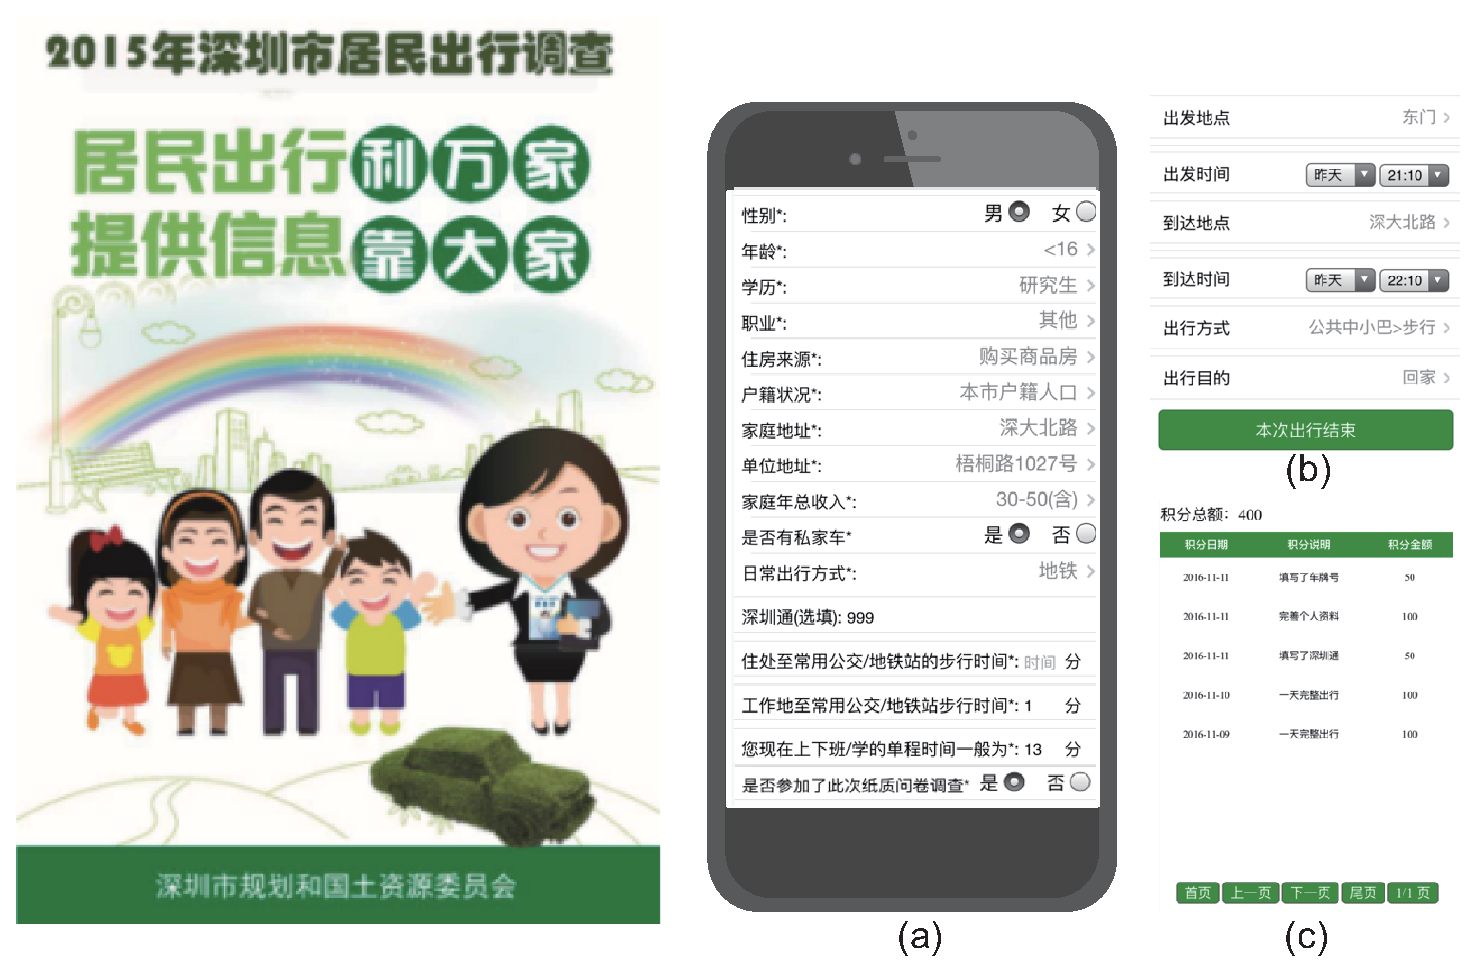
\includegraphics[width=\columnwidth]{pictures/survey_app}
 \caption{Collecting Interface: (a) welcome page; (b) personal characteristics collecting page; (c) trips collecting page; (d) credit system page}
 \label{fig:app}
\end{figure}


Over the releasing time period from June to October in 2015, 25481 individules were reached and XXX trips are collected, XX trips per individual. Figure~\ref{fig:data_over} lists the XX variables, falling into 8 domains. Those domains give a generalized depiction of the individual characteristics and serve as the ingredients for the analysis of urban dynamics over diverse people. 

Considering the caveat that self-selecting individuals are most unlikely to represent any clearly defined population~\cite{Longley2015}, a series of statistical analysis is performed to check whether it is rich enough to represent a wide range of human individuals in the city.


\begin{figure}[htb!]
 \centering % avoid the use of \begin{center}...\end{center} and use \centering instead (more compact)
 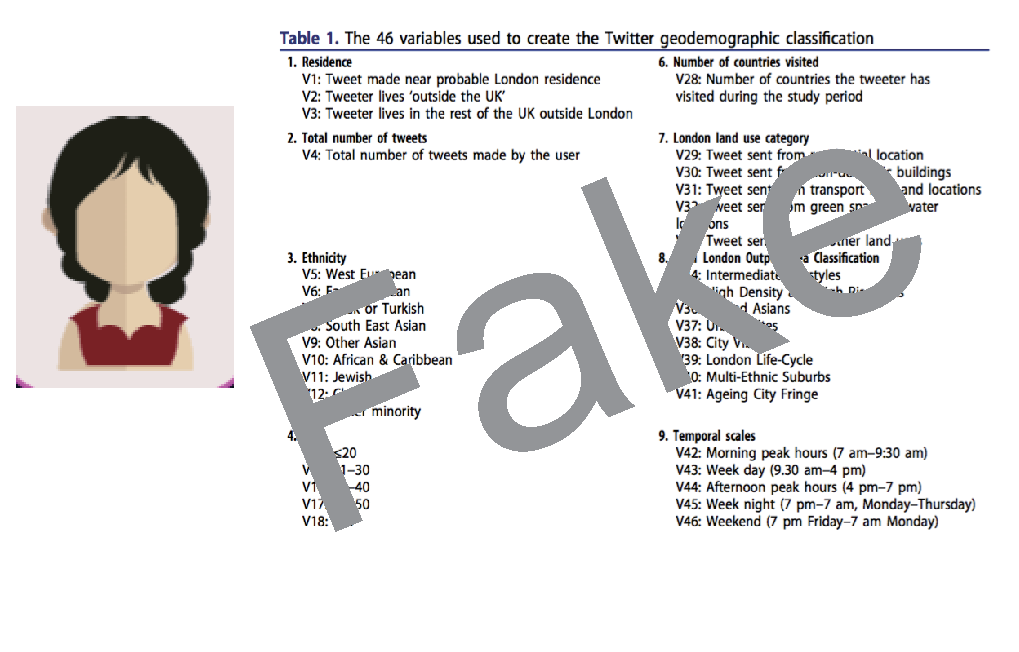
\includegraphics[width=\columnwidth]{pictures/data_over}
 \caption{Profile of Individual: XX variables falling into 8 domains enriches the analysis of urban dynamics}
 \label{fig:data_over}
\end{figure}

According to the 2015 Annual Census Statistics report~\footnote{http://www.sztj.gov.cn/xxgk/tjsj/pcgb/201606/t20160614\_3697000.htm}, people aging 15-64 occupy 83.23\% and the median age is 31.5. Shenzhen is majority of young people. 

\textit{Overview} Figure~\ref{fig:data_stat} shows samples covering almost all ages and age between 18 to 45. The 

\textit{Compared to Census} In the report (looking for some report), the penetration of mobile device is XXX, almost every XX people got a Mobile Phone in the urban. XX.  multiple social characteristics of a people is sampled, including income, education, etc. age and income distribution follows the social architecture. 


\begin{figure}[htb!]
 \centering % avoid the use of \begin{center}...\end{center} and use \centering instead (more compact)
 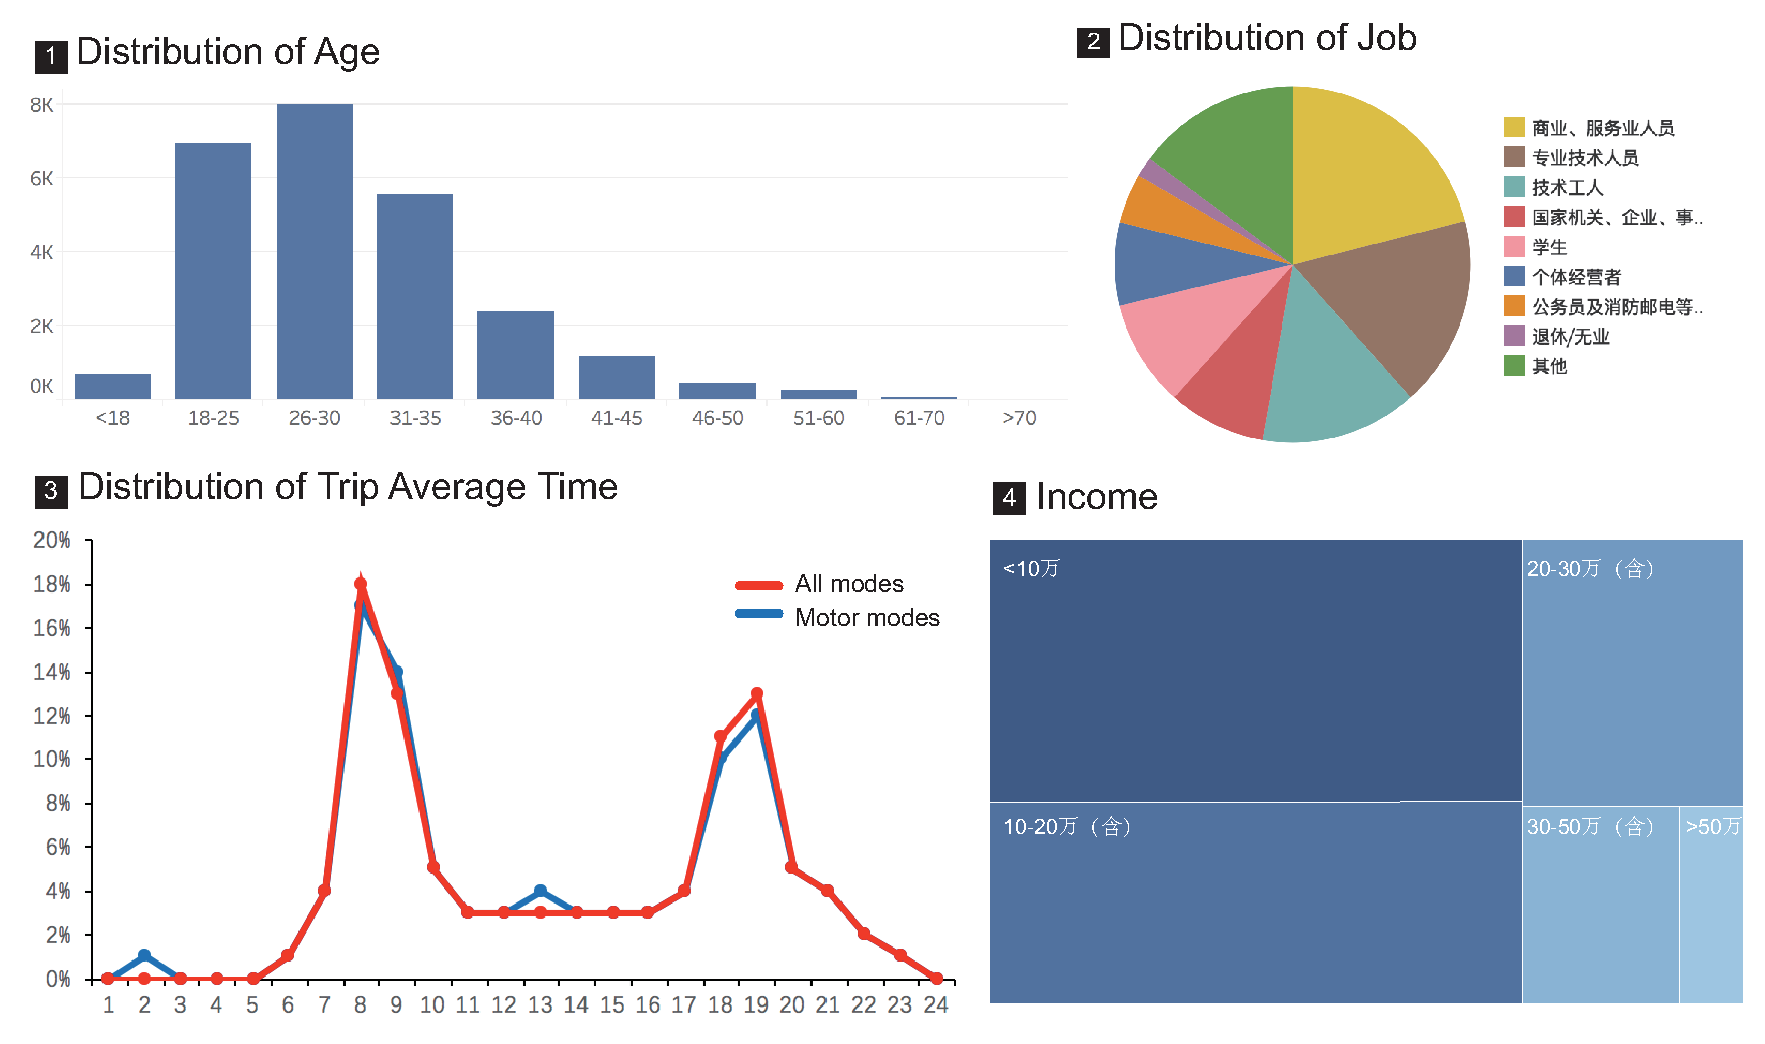
\includegraphics[width=\columnwidth]{pictures/data_detail}
 \caption{Statistical Overview of Social Characteristics}
 \label{fig:data_stat}
\end{figure}



\section{System Design}


This work we try to answer following questions:

Problem to solve: 
\begin{itemize}
\item \textit{What flows of people with certain demographic characteristics}: multiple attributes, semantic understanding, loose attribute boundary
\item \textit{What the Urban Dynamics of the Group}: where those people go and how they access the ... in a city. the patterns of behaviour classified by different social characteristics.  Including travel purpose, 
\item \textit{Compare of moving patterns between different groups}: what the similar and difference between groups in their traveling behaviour
\end{itemize}

We derive the design considerations:

\begin{itemize}
\item \textbf{C1: semantic understanding of demographic cahracteristics}: since the concept of groups is vague to define directly quantitativily. The visual design needs to consider how to help end-users to pick desirable ones from the mass. 
\item \textbf{C2: }
\end{itemize}

Classification method, flow clustering method, Semantic representation. 

The key of our work is to align the analysis of urban dynamics with the available of individual characteristics. 

Semantic understanding of social characteristics.

\subsection{Data-driven Profile Visualization}

Glyph-based visualization~\cite{borgo2013glyph} is the form of visual design to compose multivaribles into a collection of unified visual symbols, known as glyph. Glyph is intended for quick understanding and aligned comparison. Among glyph design, Chernoff Face~\cite{chernoff1973use} represents data variabules by the different features of a cartoon face. Following the idea of Chernoff Face~\cite{chernoff1973use}, we design a type of glyph, a graphical representation of people with specific demographic characteristics. The idea behind using faces is that humans easily recognize faces and notice small changes without difficulty. Those visual profiles are intended for intutive visual understanding and clustering, to abstract to concrete and semantic understanding, to help users clues to target the interested individual groups effectively.

Figure~\ref{fig:design_profile} shows the legend for the user profile. Those design dimensions are driven by data.The eight demographic dimensions are systematically designed into different visual symbols. Considering there are two types of variables, i.e., the numeric attributes and categorical attributes. By different composition, stimulus pattern which has the abstract deomgraphic measurement of individuals.

\begin{itemize}
\item \textbf{Gender} the gender is visually mapped to the hair style of the avatar. 
\item \textbf{Age} age is implied by the decoration on the hair. For the elder above 70, the hair is dyed to gray. For the youth beneath 18, hair decoration for girls and boys are adapted to the hair style.
\item \textbf{Education} The thickness of eye glasses is used to indicate the different levels in education.
\item \textbf{Job} The clothes is designed to imply the job of the individual. There are 9 types of clothes.
\item \textbf{Belongings} for house, car, residential license are considered as the belongings to the individual, so we design each of them as an add-on decoration to imply whether the individual has it or not.
\item \textbf{Income} a money symbol is used to show the different income levels.
\end{itemize} 

\begin{figure}[htb!]
 \centering % avoid the use of \begin{center}...\end{center} and use \centering instead (more compact)
 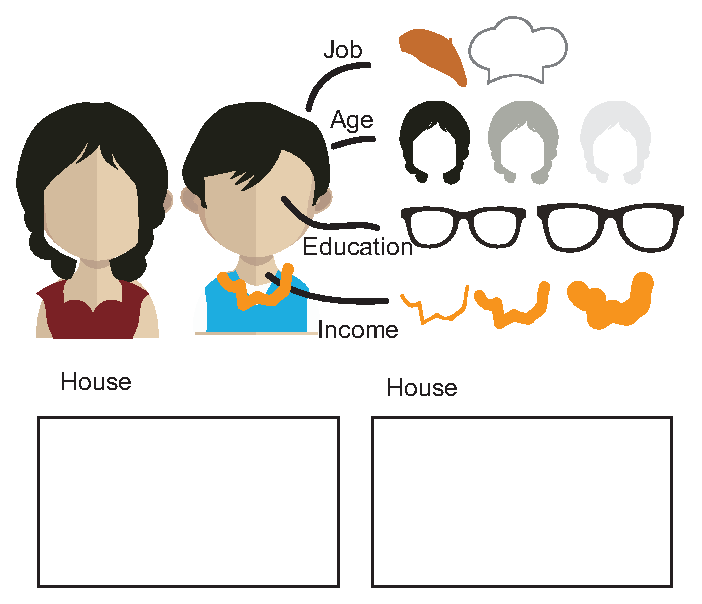
\includegraphics[width=\columnwidth]{pictures/design_profile}
 \caption{Design Profile}
 \label{fig:design_profile}
\end{figure}

With the visual mapping, the profiles varies from individual to individual. Figure~\ref{fig:div_profile} shows some examples. By concretizing the attributes which otherwise is too abstract to percept, users can scan and search for interesting target organically in figures.

\begin{figure}[htb!]
 \centering % avoid the use of \begin{center}...\end{center} and use \centering instead (more compact)
 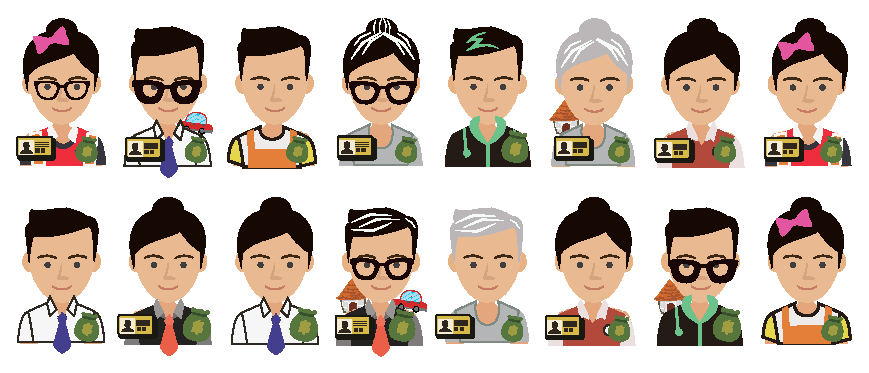
\includegraphics[width=\columnwidth]{pictures/design_div}
 \caption{Diverse Profile}
 \label{fig:div_profile}
\end{figure}

\subsection{t-SNE Projection}

Each individual is denoted as a vector with eight factors and projected as a dot into the 2D view via t-SNE project~\cite{maaten2008visualizing}, which well suits high-dimensional data for visualization in a low-dimensional space of two dimensions. As Figure~\ref{fig:tsne}(a)shows, all volunteers are embedded evenly in the 2D view, indicating the uniformly sampling over demographical space. 

Multiple views of abstract view, t-SNE proection and semantic data driven profile visualization are coordinated in a Cross-filter machinesm~\cite{Weaver2010}. It allows end-users to interactive drill-dowm into individuals with interested characteristics from multiple perspectives. Starting from the abstract criterion constraints, the scope of interest is narrowed down to individuals with(out) certian properties. And then further cross-filtering with semantically visual profiles, to check the combination of 8 characteristical variables. Figure~\ref{fig:tsne}(b) examplifies four groups of interest. 

\begin{figure}[htb!]
 \centering % avoid the use of \begin{center}...\end{center} and use \centering instead (more compact)
 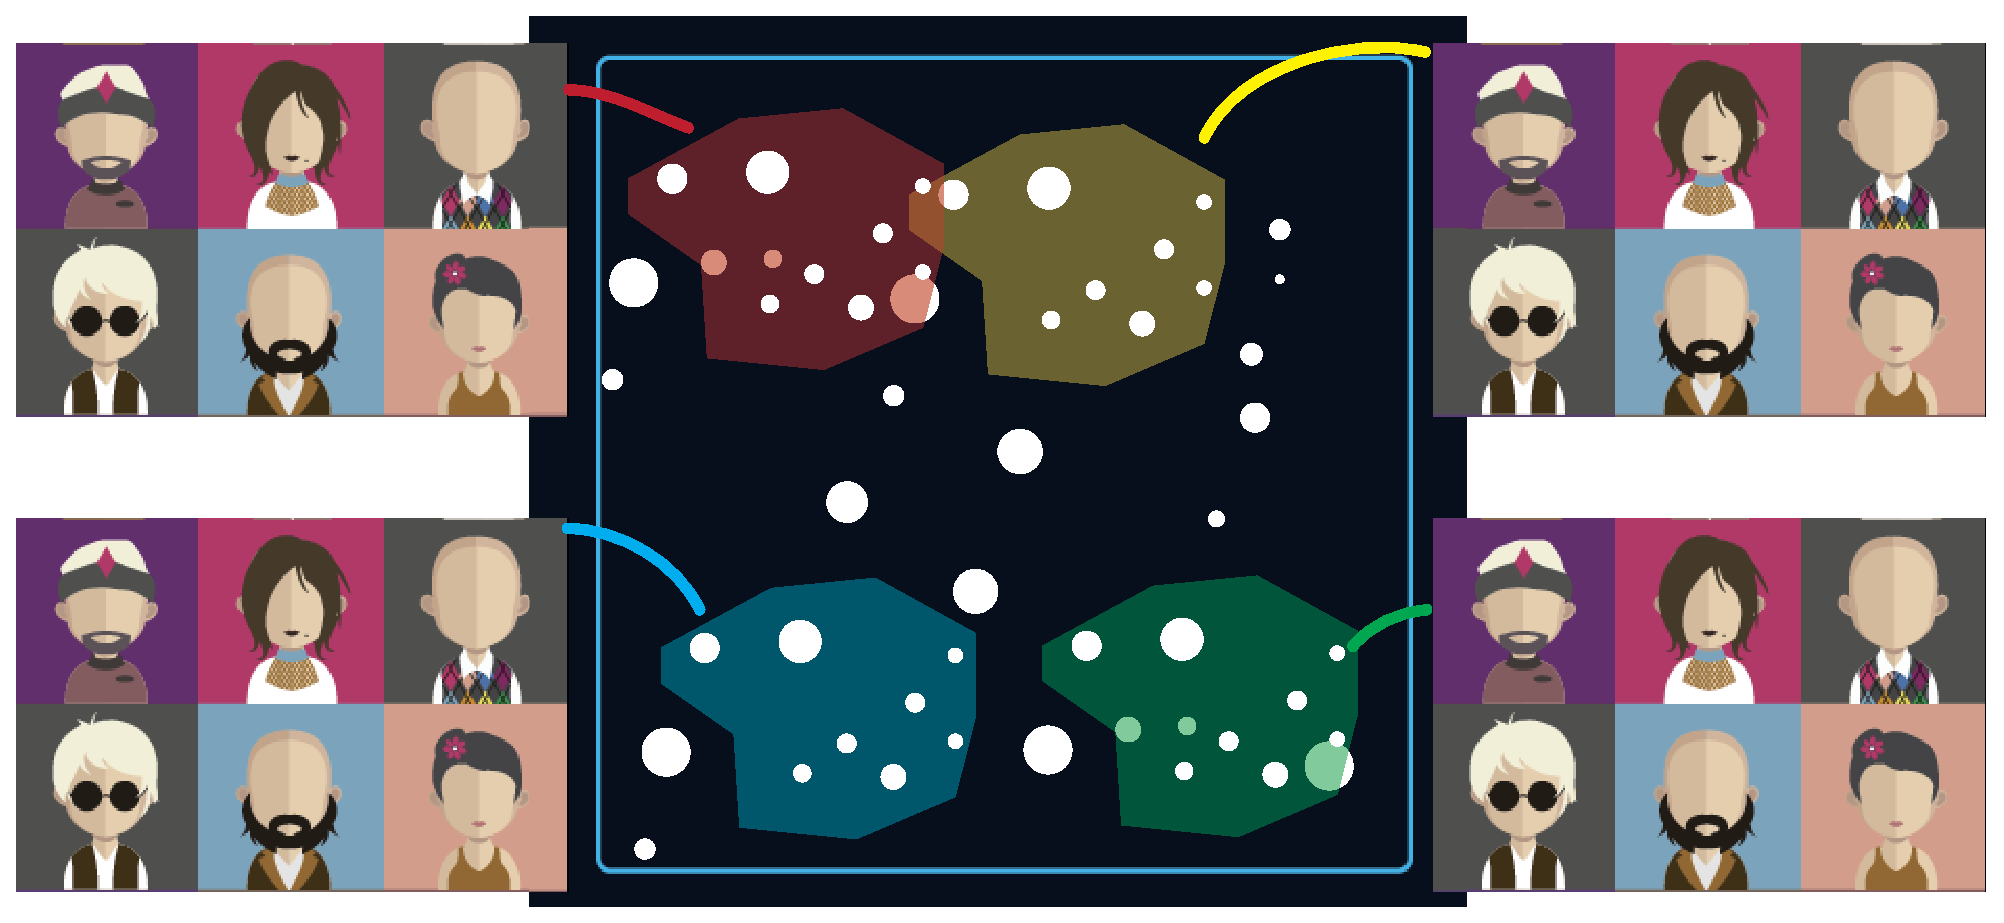
\includegraphics[width=\columnwidth]{pictures/mds}
 \caption{t-SNE project with four groups of the interest}
 \label{fig:tsne}
\end{figure}

\subsection{2.5D Spatial Visualization}

Embedding multiple variables in the spatial map is a challenging problem. Distortion technique 2D spatial, such as the partial route embedding~\cite{sun2016embedding}. However, when it comes to the global visualization, the trade-off between occlusion-free and the spatial perception. Follow the idea of 2.5D space design~\cite{Tominski2012_stacking}, the space visualization is embedded in 2.5D space, which also can smoothly transited back to the conventional 2D view.  

 Each TAZ is grown as a prism whose height encodes the occurrence of visiting. Brunch of TAZ with similar visiting pattern and purpose are grouped by an heuristic DB-Scan Algorithm in the context of TAZ. From a center TAZ, walk to neighbour TAZ to check whether aggregation or not. The aggregated TAZ brunch indicates the region visiting by the group of people in same purpose, which is often the popular traveling places. The TAZ brunch is visualized...

 To compare the mobility patterns across different groups of people, a Small Multiple dock is used to reserve the ever explored interesting result. To simply the comparion over spatial distribution, the snapshot is rendered in the 2D space, which can be magnified to check for the details in the 2.5D space.

 In this view, it supports end-users to direct manipulate the space, e.g., zooming, panning, etc. Also, detail information about the visiting can be checked by direct clicking on the TAZ. 
\section{Experts Feedback}

\lmc{Add a section to introduce the domain experts' feedback}


\lm{We interview XX domain experts from the GIS field. XX of them are with ... The procedure went as following. We first introduce them the system an...}

\section{Case Study}

Applied the system to Shenzhen's dataset. We demonstrate the efficiency. 

\subsection{OVERVIEW Case 1: City Folding}

compare the distorted maps from various groups

Different different groups of people and see their patterns across the city.

Group 1 is defined as xxxxx. The popular visiting places

Wealthier people with better access to ... than poor people. 

\subsection{DETAIL Case 2: Look into Detail}

check the detail information of a group

To compare the Group 1 and Group 2, the similar places and different places...
% \section{Discussion}

\textbf{Compatibility}

Compared to other static visual cuing, animation effect has better compatibility by not importing other markers. 

\textbf{Mapping}

Kinetic effects is driven by data with what kind of mapping, linear, non-linear? relationship to perceptual driven, tuned by perception. 


\textbf{Visual Tired/ Distracting the reading of other visual channel}

 Does it disturb the reading of original static charts?
 
 What we show in this work is to add kinetic effect all in, the extreme case of visual information enhancement. If applying to certain part of visual objects, it would for sure significantly reduce the visual distraction and facilitate the attention attraction.
  
\textbf{Interactive Enhancement / Adaptive Dynamic Control}

For sure the kinetic effects can be used in the interactive visual analytics system, as the cuing techniques after interactions, e.g., annotation, filtering, query, etc. For most of visual analytics, existing visual cuing is static and because of buried in rich visual encoding, it is usually hard to stand out. Kinetic effects can be considered as efficient attention attraction encoding. 

Also, it also allows the users' manual control on playing/stopping kinetic effect, to call the enhancement of information on demand

Adaptive dynamic enhancement, e.g., sleep the kinetic effects ?



\section{Conclusion}

In this paper, we presented the map distrotion, whis driven by the accessibility of demographics. Our experimental findings indicate that ..., that aids in ...

Our current ...


 


% In this work, we propose to enhance static charts with kinetic effects, which serve as an plausible and orthogonal extension of conventional static visual cuing. Three kinetic effects (marching ants, geometry deformation and blinking) are introduced to demonstrate the idea from dynamic effects of motion, deformation and on-off repeating patterns. Kinetic effects encode various messages by design dimensions via the data driven mechanism. ...  kinetic effects brings the unsaid or less-notified information and bring the static infographics and charts to life. A controlled user study ...%Aligned with daily life experience , charts  enhanced by Kinetic Effect provides 
% which maintains the richness of expressibility . 


%% if specified like this the section will be committed in review mode
% \acknowledgments{
% The authors wish to thank A, B, and C. This work was supported in part by
% a grant from XYZ (\# 12345-67890).}

%\bibliographystyle{abbrv}
\bibliographystyle{abbrv-doi}
%\bibliographystyle{abbrv-doi-narrow}
%\bibliographystyle{abbrv-doi-hyperref}
%\bibliographystyle{abbrv-doi-hyperref-narrow}

\bibliography{main}
\end{document}

